	\clearpage
\section{Konzept}\label{sec:Konzept}

Für den Vergleich der 3 Mesh Netzwerkstack Bluetooth Mesh (BT Mesh), Thread und Zigbee soll folgendes vom Protokoll unabhängiges Testkonzept umgesetzt werden. 
Die Abbildung \ref{fig:MeshTestKonzept} zeigt das Konzeptschema. Die Benchmark Slave Nodes (BSN) in der Abbildung als Sensoren und Aktoren mit unterschiedlichen Funktionalitäten dargestellt, bilden zusammen mit dem Benchmark Master Node (BMN) das zu testende Mesh Netzwerk. Innerhalb des Netzwerks wird dessen Organisation vom jeweiligen Protokoll sichergestellt. 
Die Benchmark Management Station (BMS) welche mit dem BMN via USB/UART kommuniziert ist zuständig für die Verwaltung und Verarbeitung der Benchmarks. Während eines Benchmark Prozesses sollen sämtliche Messungen jedoch unabhängig von der BMS durchgeführt werden damit allfällige Latenzzeiten der USB/UART Verbindung die Resultate nicht verfälschen.
Das Mesh Testnetzwerk soll unter unterschiedlichen Bedingungen betrieben. Diese Testszenarien werden unter \ref{sec:Testszenarien} genauer beschrieben.


\begin{figure}[H]
	\centering
	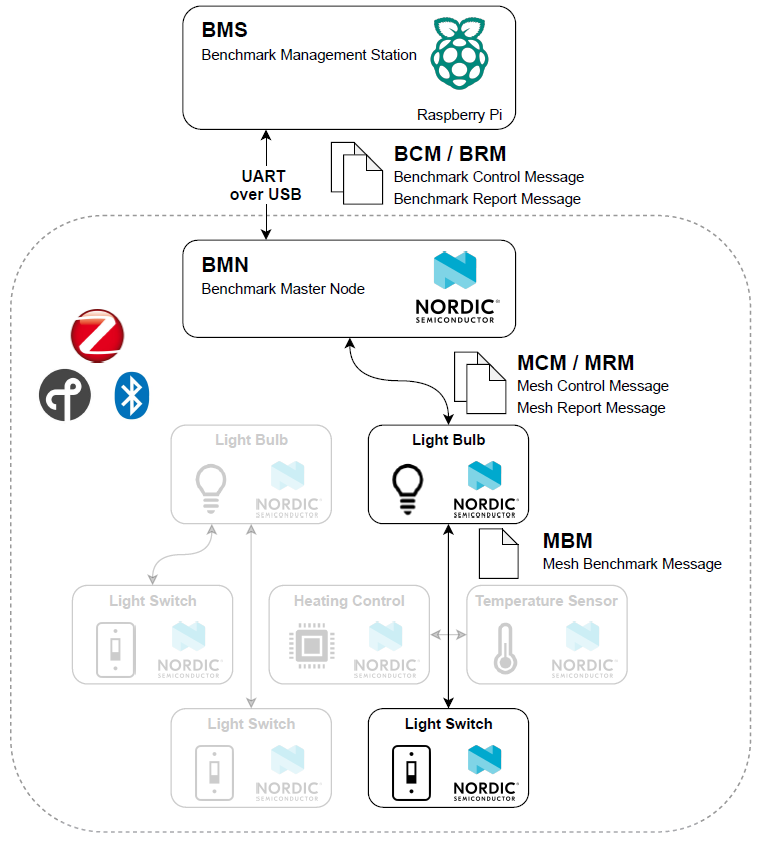
\includegraphics[width=1.0\textwidth]{Mesh_Testkonzept.png}
	\caption{Konzeptschema für den Ablauf eines Mesh Benchmarks.}\label{fig:MeshTestKonzept}
\end{figure}


\todo[inline]{RAN: Beschreibung Graphik einfügen}

\subsection{Mesh Benchmark Message (MBM)}\label{subsec:MeshBenchmarkMessage}
Die MBM ist jene Message welche die eigentlichen Messdaten produziert und diese sogleich unter den BSN (Mesh Knoten) überträgt. Anhand dieser Message werden die Parameter gemäss der Kennwerttabelle in Anhang xx erfasst.

\todo[inline]{Achtung Dummy Bild ;-)}

\begin{figure}[H]
	\centering
	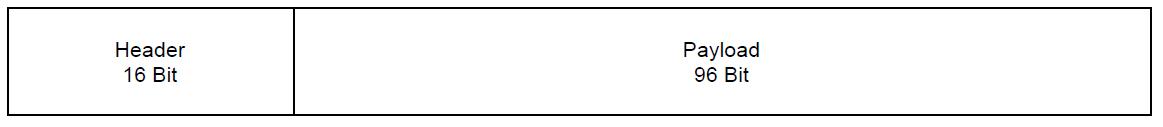
\includegraphics[width=1.0\textwidth]{MeshBenchmarkMessagePaketdefinition.png}
	\caption{Packet Definition der Mesh Benchmark Message (MBM)}\label{fig:MeshTestKonzept}
\end{figure}


\subsection{Mesh Control Message (MCM)}\label{subsec:MeshControlMessage}


\todo[inline]{Achtung Dummy Bild ;-)}

\begin{figure}[H]
	\centering
	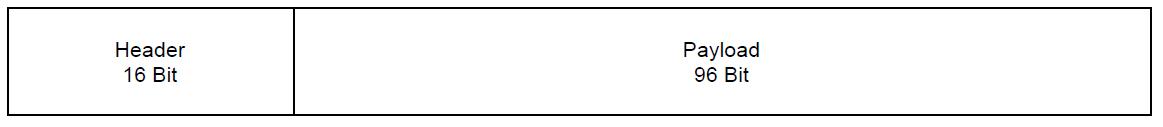
\includegraphics[width=1.0\textwidth]{MeshControlMessagePaketdefinition.png}
	\caption{Packet Definition der Mesh Control Message (MCM)}\label{fig:MeshTestKonzept}
\end{figure}

\subsection{Mesh Report Message (MRM)}\label{subsec:MeshReportMessage}


\todo[inline]{Achtung Dummy Bild ;-)}

\begin{figure}[H]
	\centering
	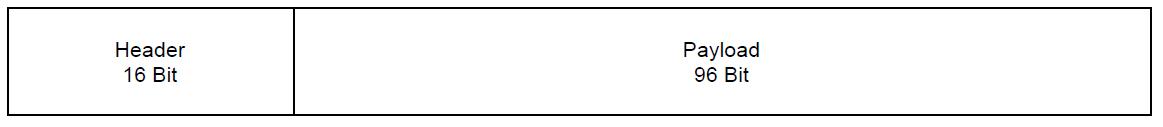
\includegraphics[width=1.0\textwidth]{MeshReportMessagePaketdefinition.png}
	\caption{Packet Definition der Mesh Report Message (MRM))}\label{fig:MeshTestKonzept}
\end{figure}

\subsection{Benchmark Control Message (BCM)}\label{subsec:BenchmarkControlMessage}

\todo[inline]{Achtung Dummy Bild ;-)}

\begin{figure}[H]
	\centering
	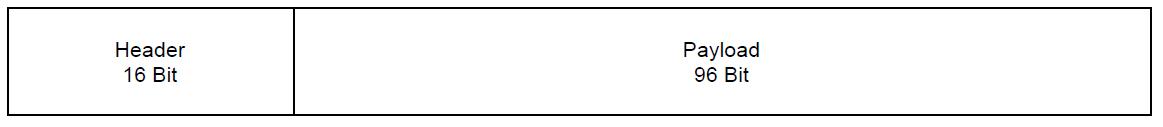
\includegraphics[width=1.0\textwidth]{BenchmarkControlMessagePaketdefinition.png}
	\caption{Packet Definition der Benchmark Control Message (BCM)}\label{fig:MeshTestKonzept}
\end{figure}

\subsection{Benchmark Report Message (BRM)}\label{subsec:BenchmarkReportMessage}

\todo[inline]{Achtung Dummy Bild ;-)}

\begin{figure}[H]
	\centering
	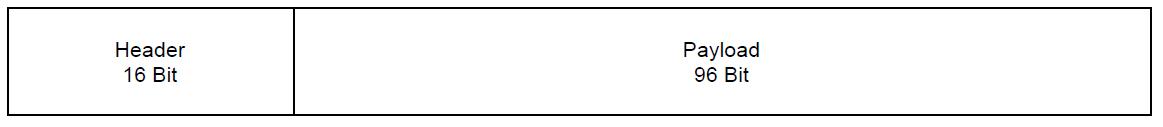
\includegraphics[width=1.0\textwidth]{BenchmarkReportMessagePaketdefinition.png}
	\caption{Packet Definition der Benchmark Report Message (BRM)}\label{fig:MeshTestKonzept}
\end{figure}


